\chapter{Вимірювання імпедансу за допомогою HP4192a} 
\label{chap:first}

У цій частині ми вчились приборкувати \sout{дракона} імпедансметр HP4192a. У нас було 3 завдання: дослідити залежність імпедансу від частоти для резистора, конденсатора та котушки.

\section{Вимірювання активного та реактивного опору резистора}

Отримана експеримантальним шляхом залежність активного та реактивного опору резистора від частоти (рис. \ref{fig:part221}) не викликає сумнівів. Справді, активний опір не залежав істотно від частоти, та був приблизно рівним $95.4 \Omega$ упродовж всього експерименту. На рахунок реактивного опору - при високих частотах опір явно росте, що викликано індуктивними властивостями дротів, використаних у цьому резисторі. При малих частотах реактивний опір також росте, однак це вже викликано тим, що наш резистор в деякому сенсі працює як конденсатор.

\begin{figure}[h]
    \begin{minipage}[h]{0.47\linewidth}
        \center{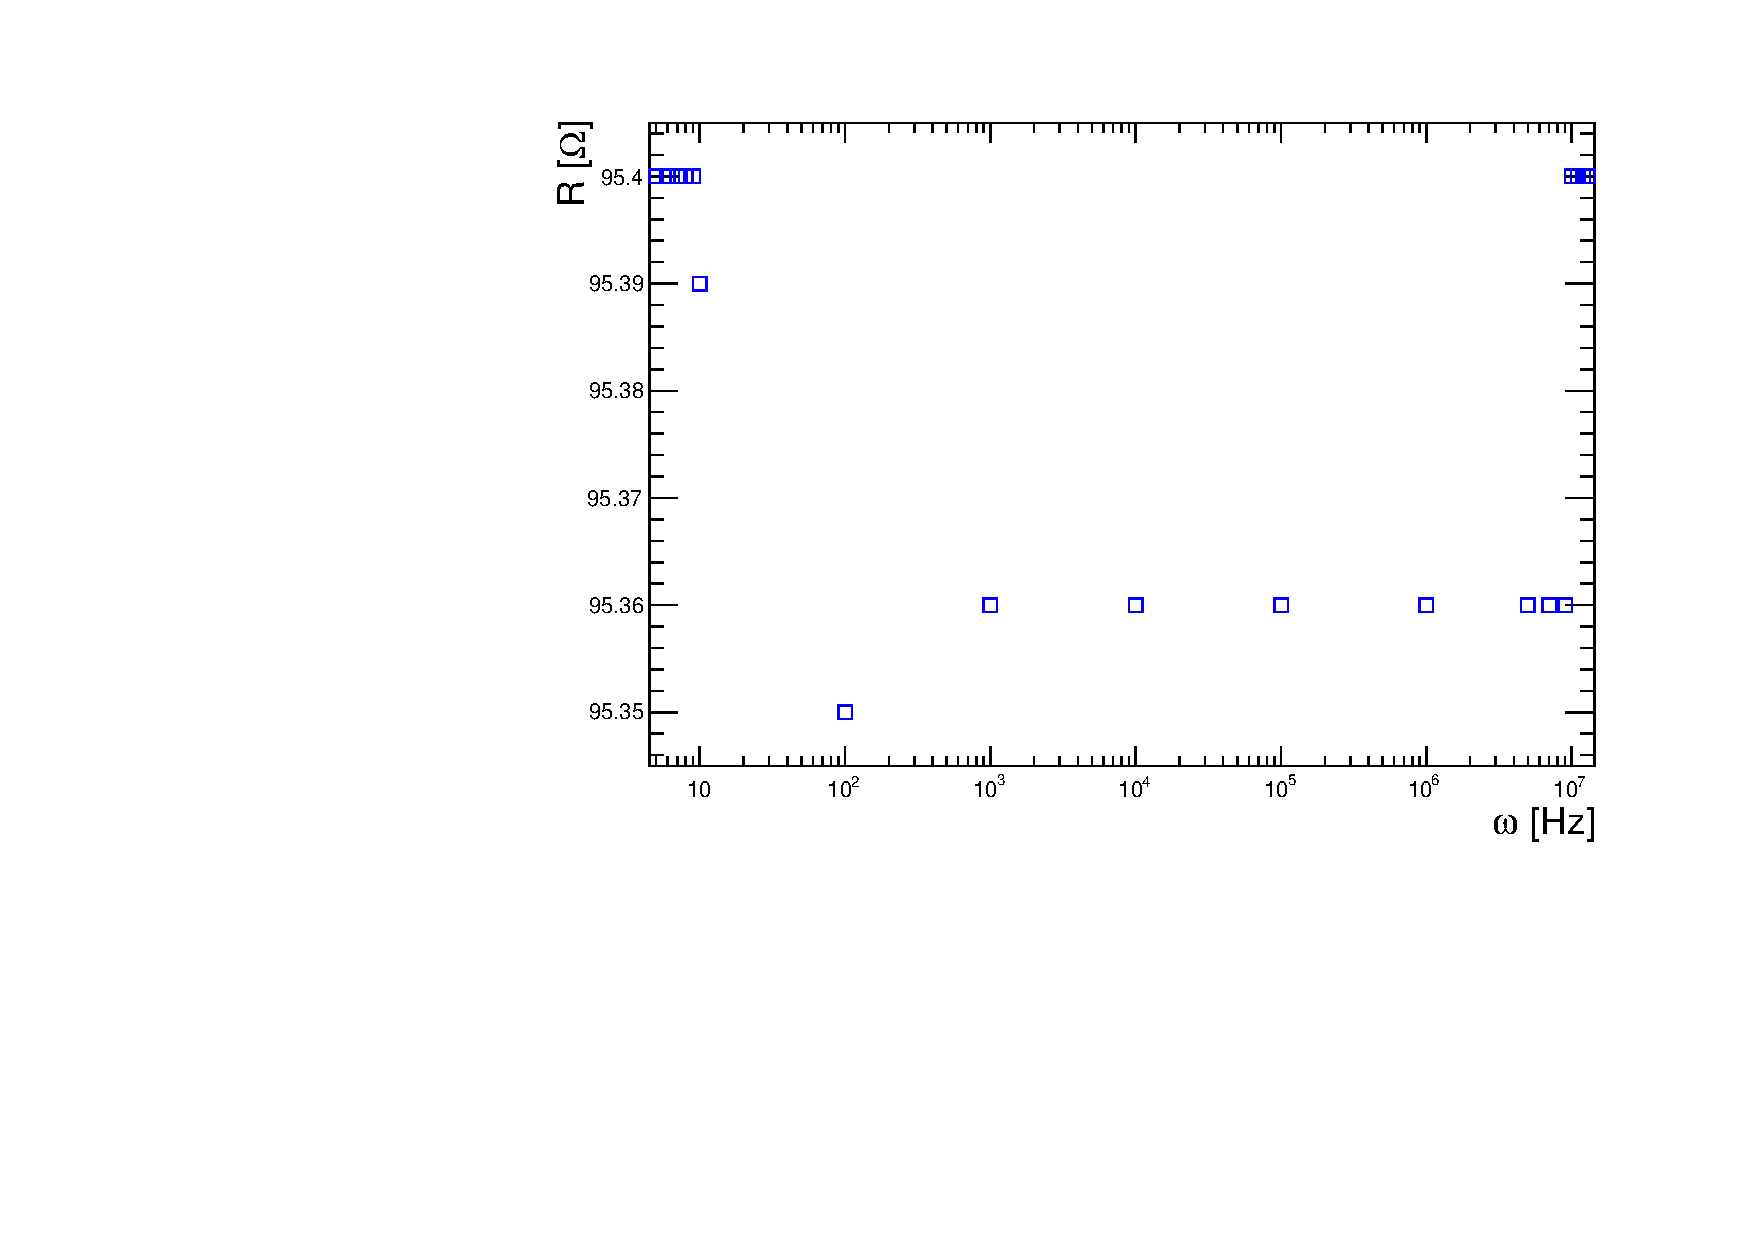
\includegraphics[width=1\linewidth]{pdf/c1_RR.pdf}} \\
    \end{minipage}
    \hfill
    \begin{minipage}[h]{0.47\linewidth}
        \center{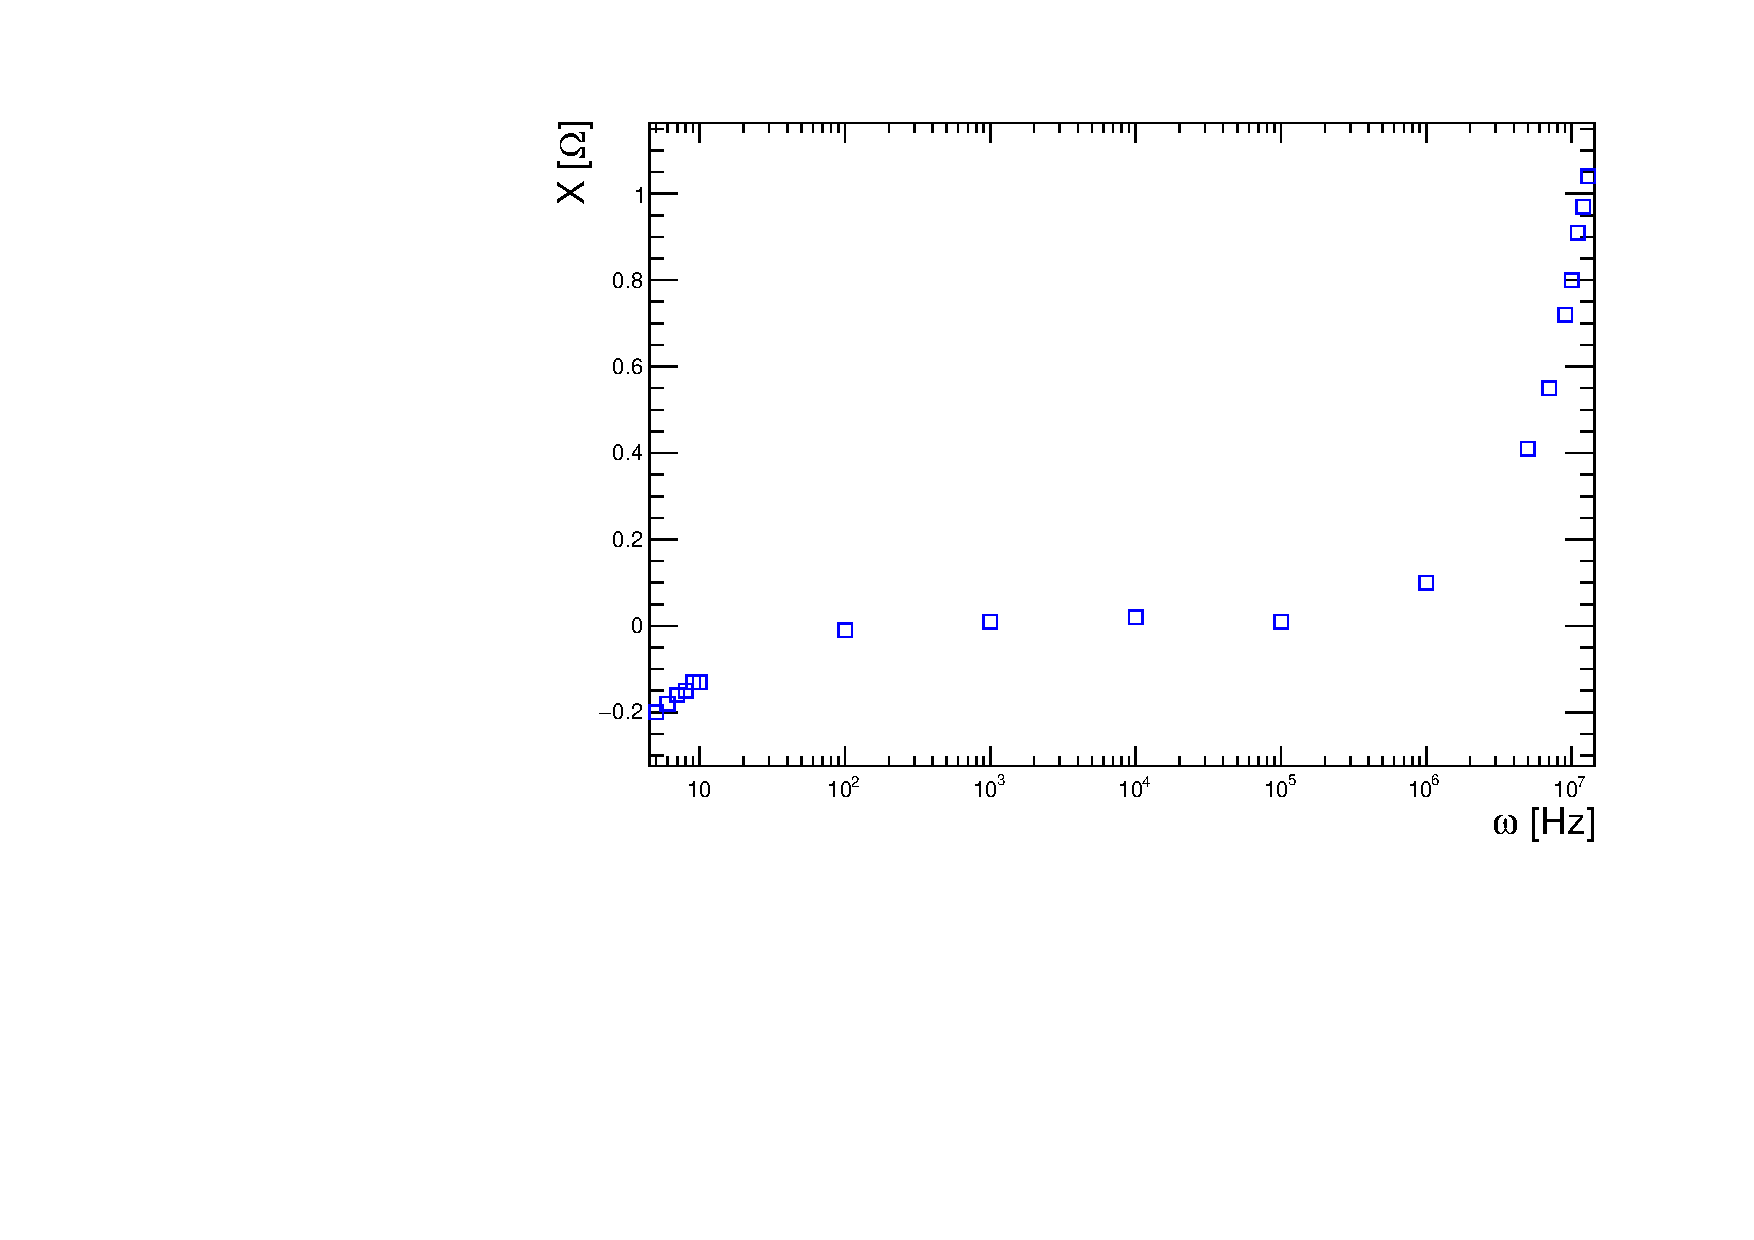
\includegraphics[width=1\linewidth]{pdf/c1_RX.pdf}}\\
    \end{minipage}
    \caption{Залежність активного та реактивного опору резистора від частоти}
    \label{fig:part221}
\end{figure}


\section{Вимірювання активного та реактивного опору конденсатора}

Отримана експеримантальним шляхом залежність активного та реактивного опору конденсатора від частоти (рис. \ref{fig:part222}) виявилась досить цікавою. Справді, активний опір досить швидко обвалюється, що природньо, однак при $\omega \approx 10^7 Hz$ має досить дивний пік, що можливо пов'язано із властивостями діалектрика всередині. Реактивний опір спочатку спадає, тобто поводить себе як в ідеальному конденсаторі, маючи мінімум при частоті $\omega \approx 10^5 Hz$, яка є власною резонансною частотою. Проте після цього опір починає збільшуватися, що пояснюється зростанням паразитної індуктивності, яка і визначає імпеданс конденсатора на високих частотах. Відповідна поведінка реактивного опору корелює із залежністю ємності від частоти \ref{fig:part2C}, що має спочатку поличку (область ідеального конденсатора), потім сингулярність у зоні резонансу, і після прямування до нуля, що наглядно показує те, шо при високих частотах ємнісні властивості конденсатора поступаються паразитним індуктивностям. Для обчислення ємності використовувалася формула: $C = \frac{1}{X(\omega)\omega}$.

\begin{figure}[h]
    \begin{minipage}[h]{0.47\linewidth}
        \center{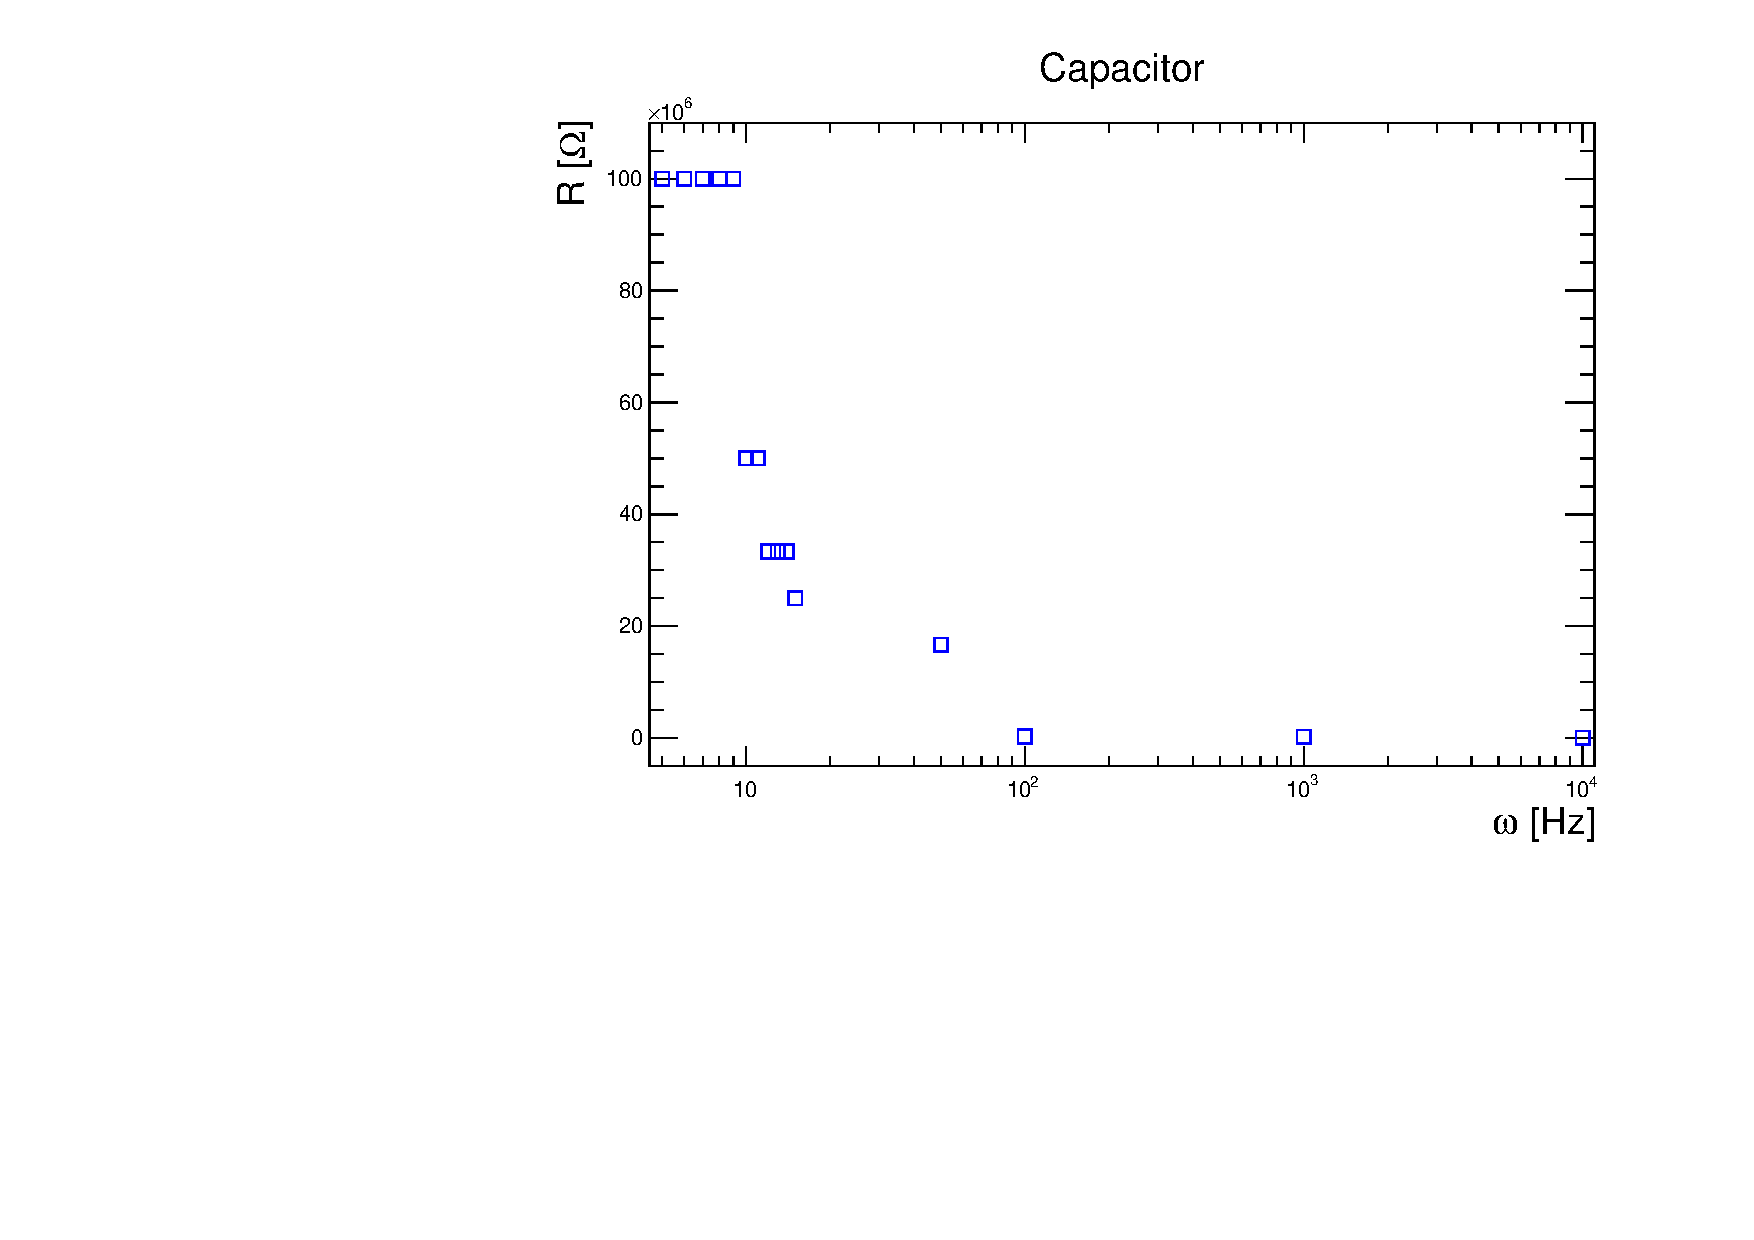
\includegraphics[width=1\linewidth]{pdf/c1_CR.pdf}} \\
    \end{minipage}
    \hfill
    \begin{minipage}[h]{0.47\linewidth}
        \center{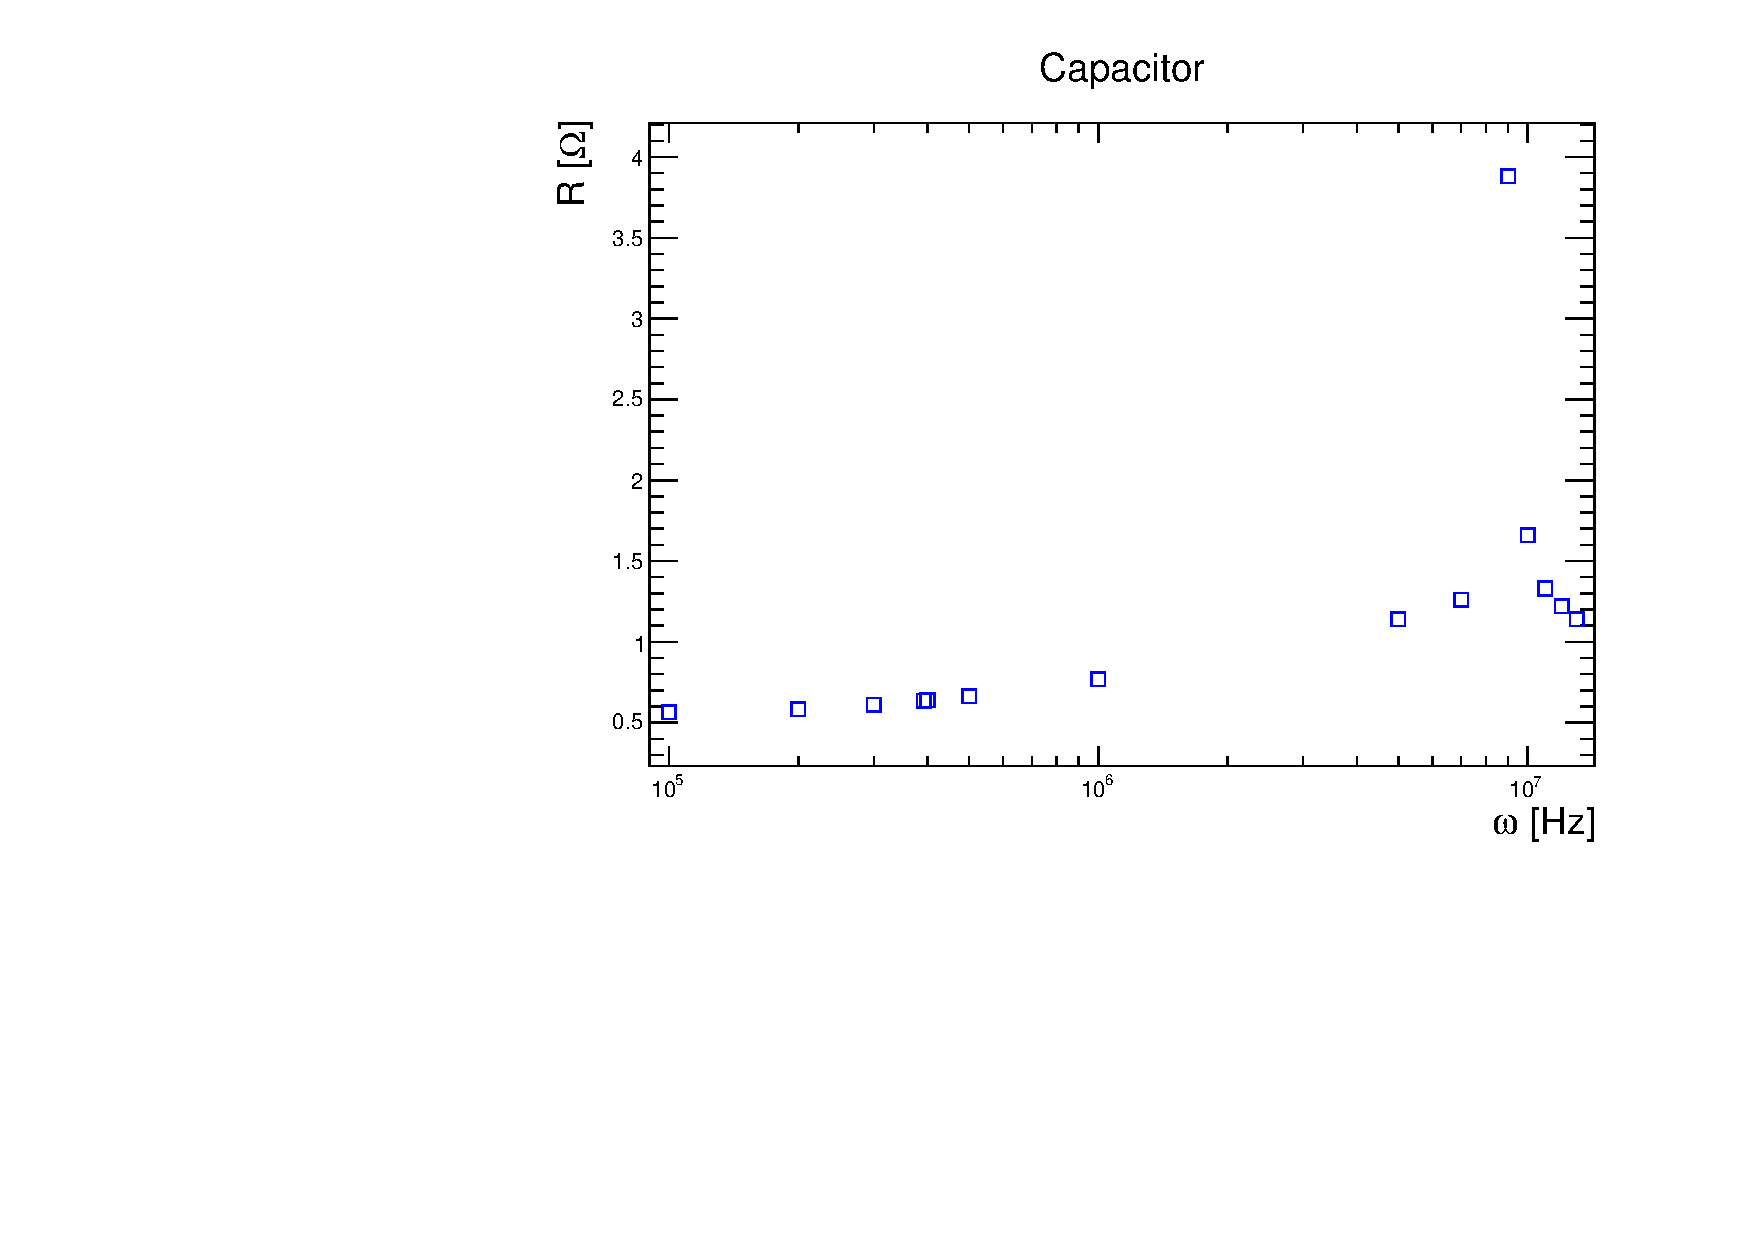
\includegraphics[width=1\linewidth]{pdf/c1_CR2.pdf}}\\
    \end{minipage}
    \vfill
    \begin{minipage}[h]{0.47\linewidth}
        \center{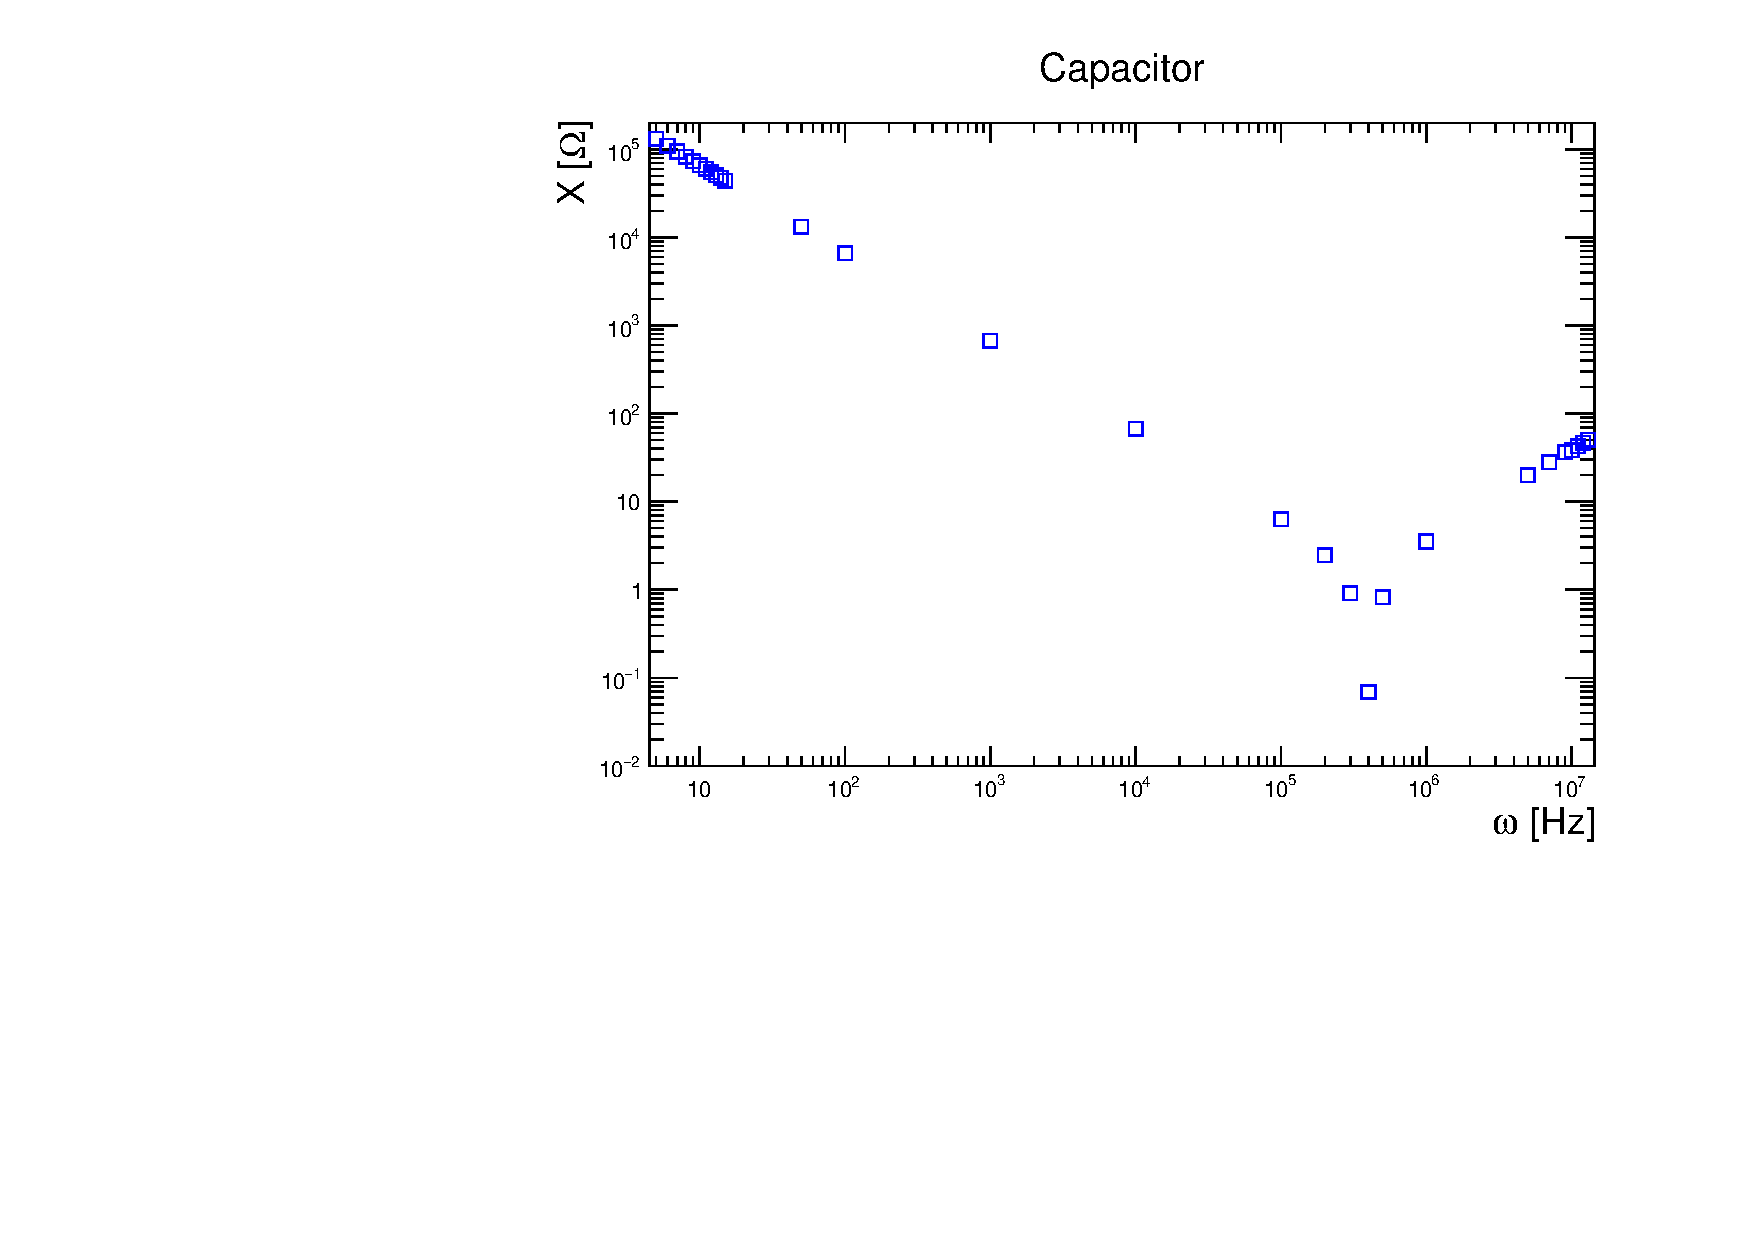
\includegraphics[width=1\linewidth]{pdf/c1_CX.pdf}}\\
    \end{minipage}
    \caption{Залежність активного та реактивного опору конденсатора від частоти}
    \label{fig:part222}
\end{figure}

\begin{figure}[h]
    \center{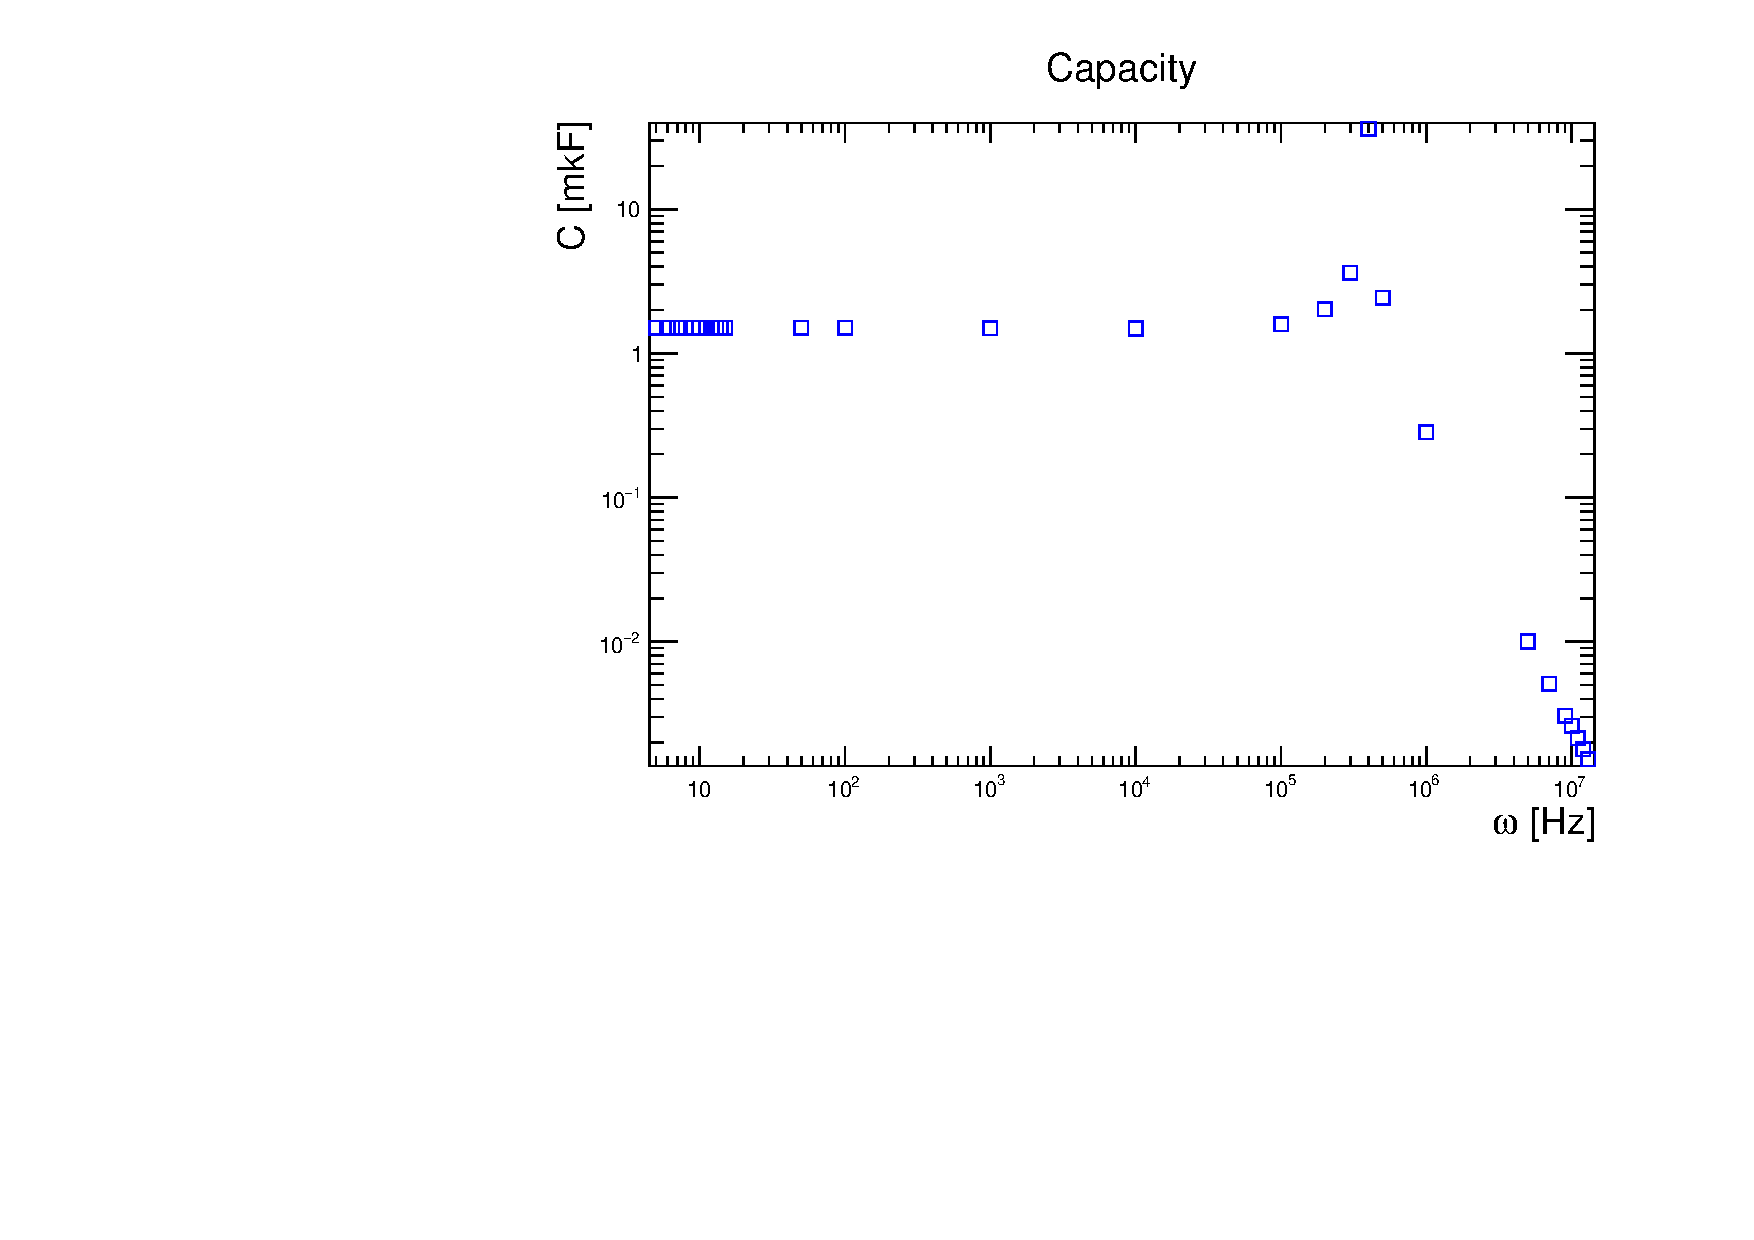
\includegraphics[width=0.45\linewidth]{pdf/c1_C_omega.pdf}} \\
    \caption{Залежність ємності конденсатора від частоти.}
    \label{fig:part2C}
\end{figure}

\section{Вимірювання активного та реактивного опору котушки}

Отримана експеримантальним шляхом залежність активного котушки від частоти (рис. \ref{fig:part223}) викликає бажання у автора спитати викладача про доцільність даного експерименту. Справді, поведінка активного опору може бути охарактеризована прекрасною фразою брєд сивої кобили. Хоча пік реактивного опору в районі $\omega \approx 10^6 Hz$, після якого імпеданс котушки з індуктивного стає ємнісним виглядає досить цікавим. Пояснення цього явища виявилось досить простим: оскільки жодний фізичний прилад не можна вважати ідеальним, то котушка проявляє себе на певній частоті (її називають власною частотою даної котушки індуктивності) як схема RLC елементів.(рис. \ref{fig:ssanahuina}) Прийнято вважати, що ємність виникає між витками котушки і створює спостережуваний ефект, а опір пояснює певні втрати на даному елементі.\cite{huina}.

\begin{figure}[h]
    \begin{minipage}[h]{0.47\linewidth}
        \center{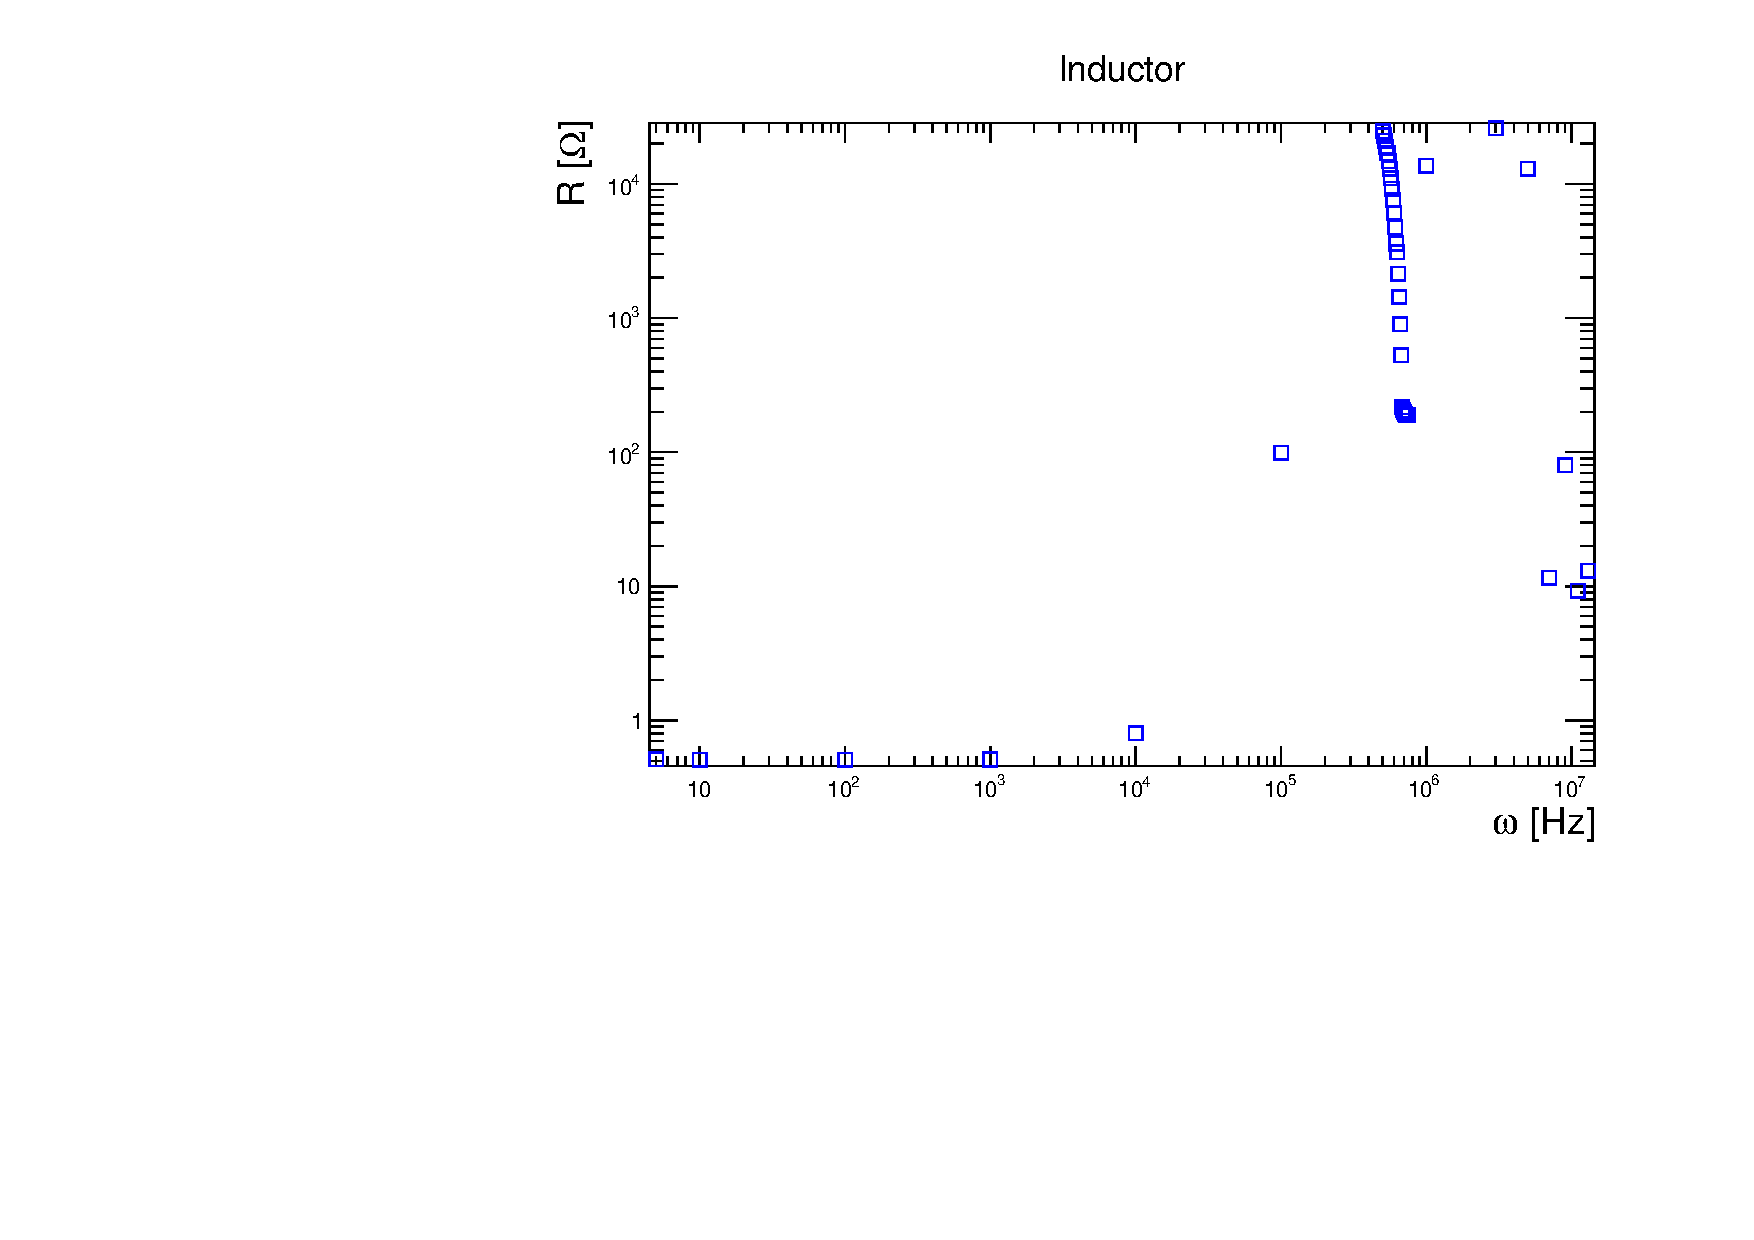
\includegraphics[width=1\linewidth]{pdf/c1_LR.pdf}} \\
    \end{minipage}
    \hfill
    \begin{minipage}[h]{0.47\linewidth}
        \center{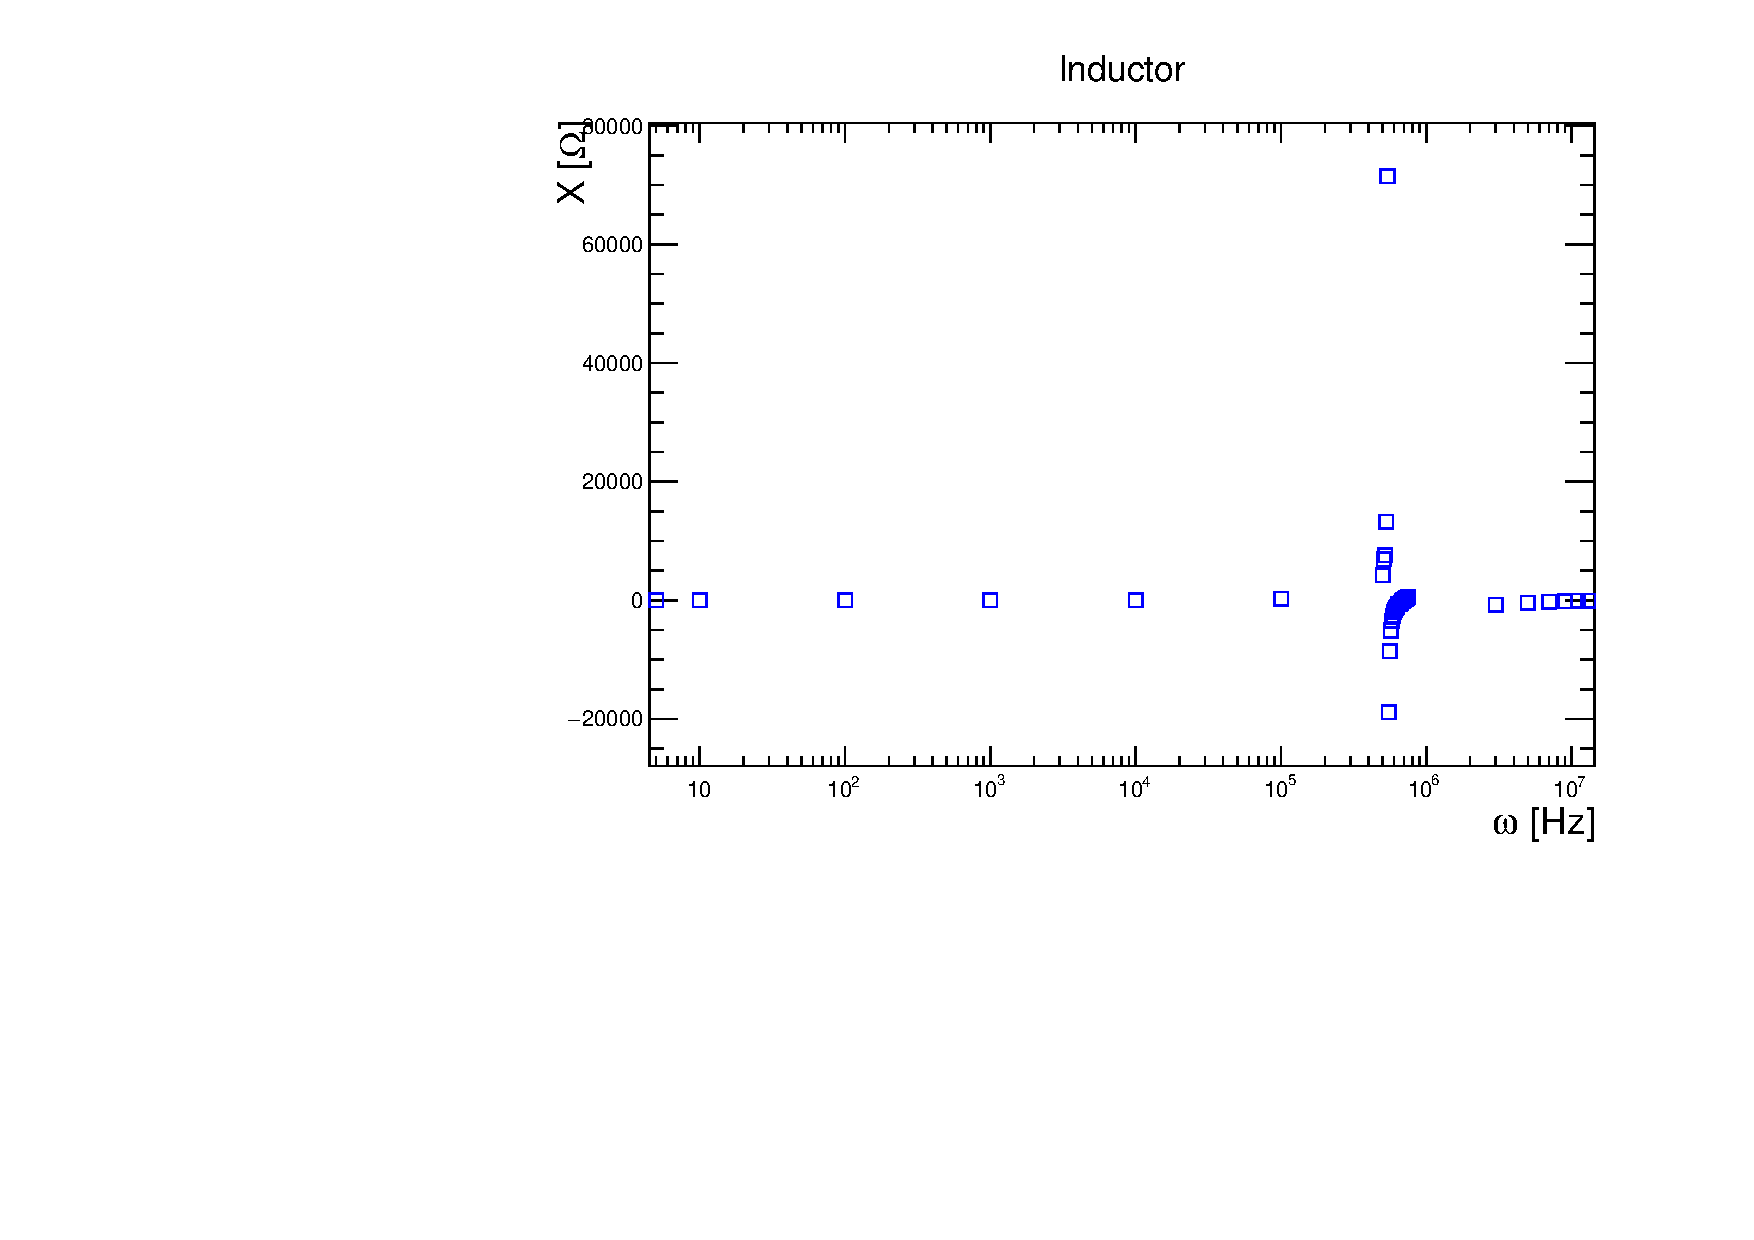
\includegraphics[width=1\linewidth]{pdf/c1_LX.pdf}}\\
    \end{minipage}    
    \caption{Залежність активного та реактивного опору котушки від частоти}
    \label{fig:part223}
\end{figure}

\begin{figure}[h]
    \center{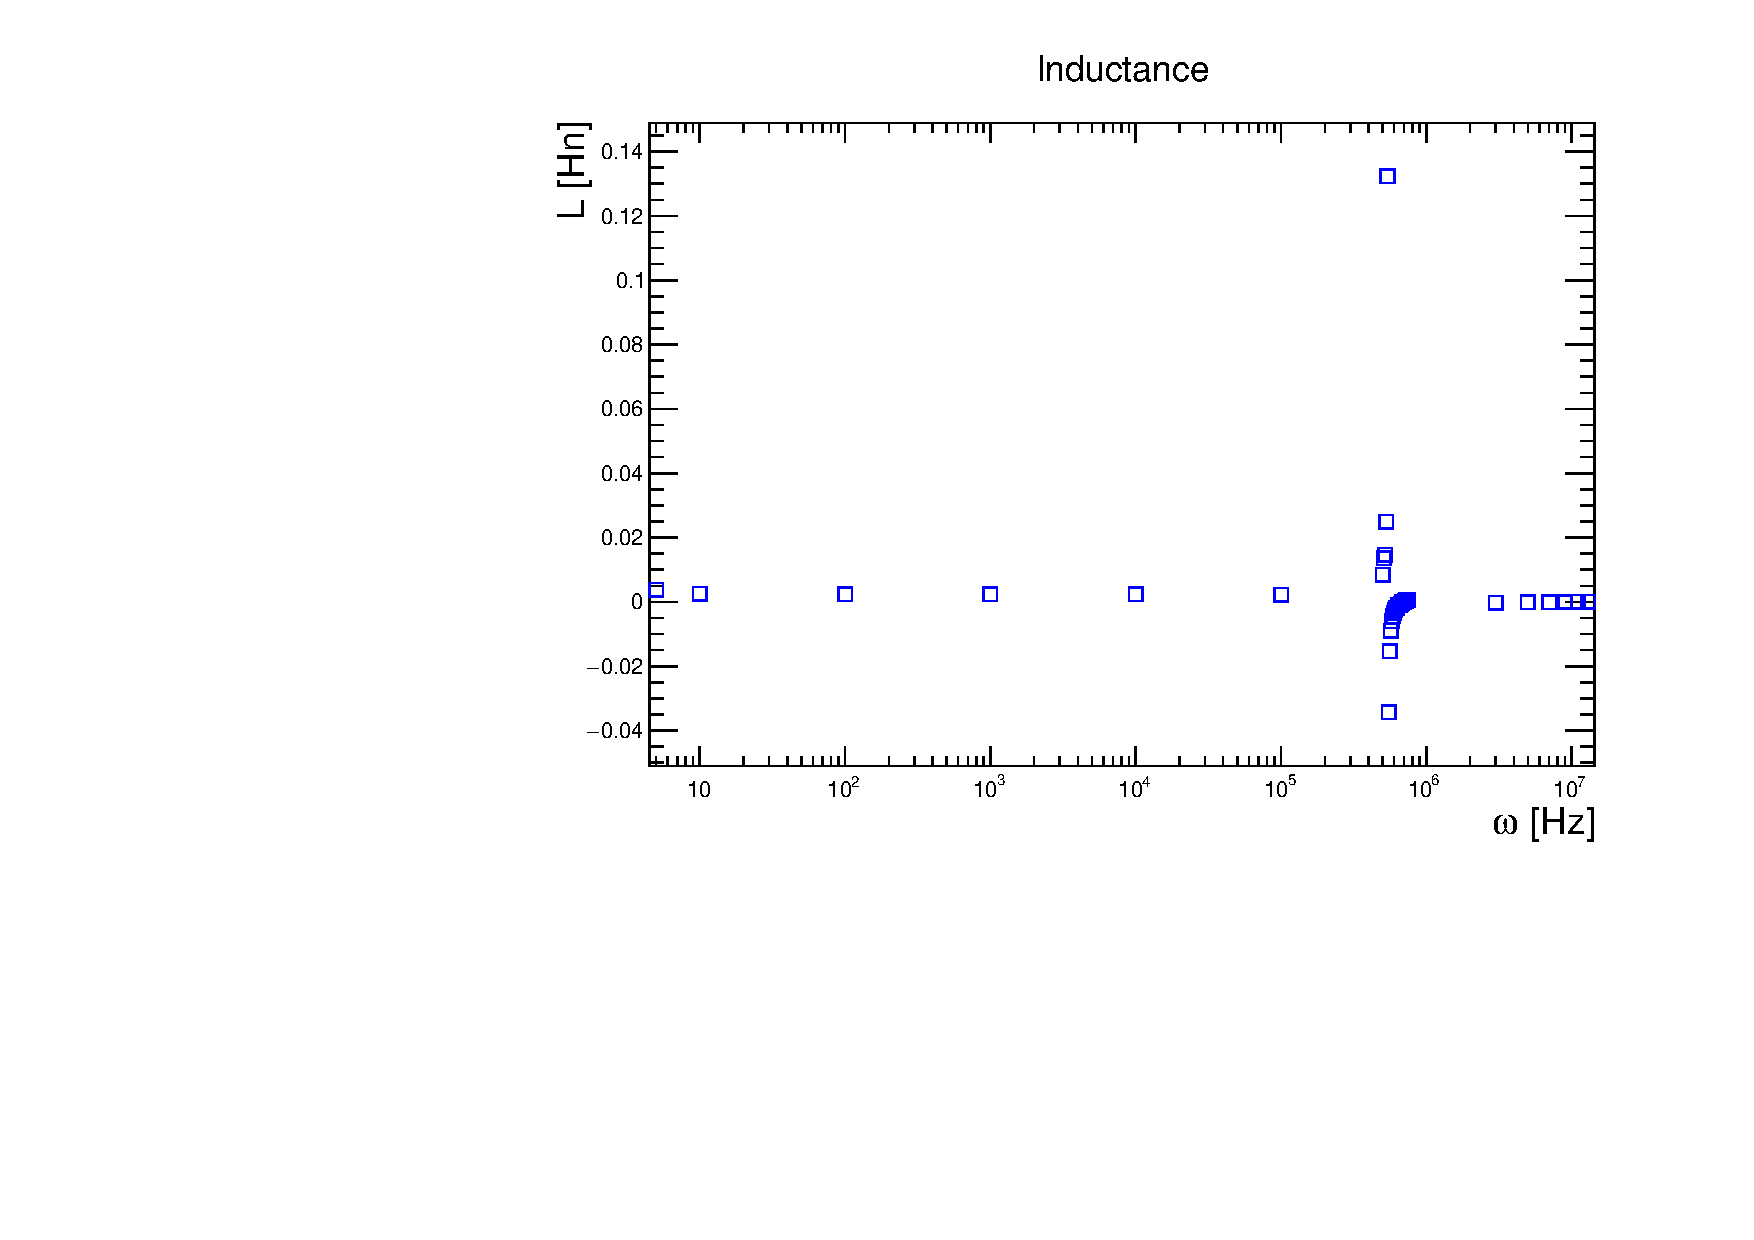
\includegraphics[width=0.45\linewidth]{pdf/c1_L_omega.pdf}} \\
    \caption{Залежність індуктивності котушки від частоти.}
    \label{fig:part3L}
\end{figure}

Відповідно до теорії веде себе і індуктивність: константа при малих частотах, сингулярність в області резонансу, та прямування до нуля при високих частотах \ref{fig:part3L}. Цікаво, що графік її залежності майже повністю повторює вигляд реактивного опору від частоти.

\begin{figure}[h]    
        \center{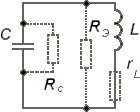
\includegraphics[width=0.3\linewidth]{contecv.png}} \\
    \caption{Представлення котушки як схеми RLC елементів}
    \label{fig:ssanahuina}
\end{figure}

Взагалі, робота з даним приладом варта 2 пострілам в голову, адже випадковим чином підібрані знаки, та інколи числа на його екрані не дають в спокійному режимі зняти потрібні покази.